\chapter{Related work}
This chapter explains the necessary basis to understand the procedure and contains all relevant information of previous work in this field.

% AI
% Finetuning / Transfer Learning
% Modern approaches: Lora, Adapter
% Frozen evaluation
% Utility Score

\section{Models}

\subsection{Resnet50}
Figure~\ref{fig:resnet50_architecture}.

\begin{figure}[H]
    \begin{center}
    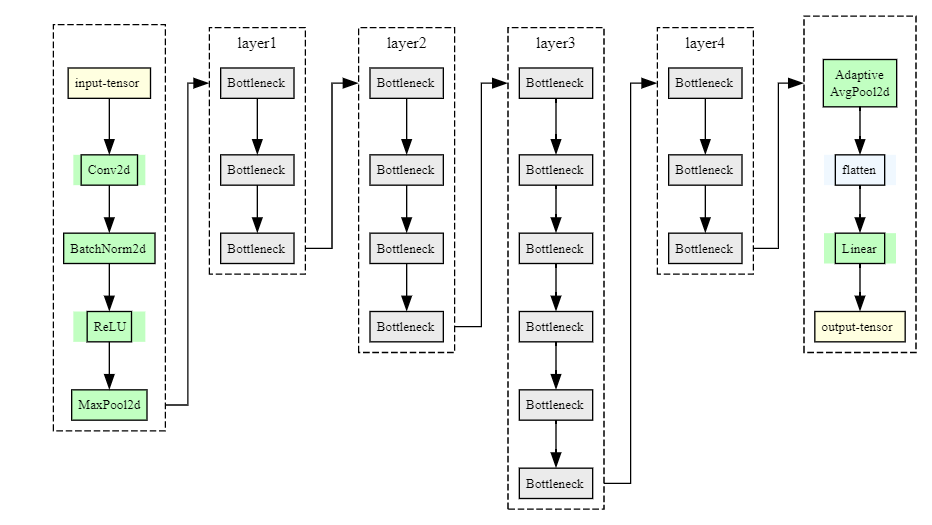
\includegraphics[width=15cm]{../images/resnet50_architecture.png}
    \caption{Architecture of Resnet50}
   \label{fig:resnet50_architecture}
    \end{center}
\end{figure}

Figure~\ref{fig:resnet50_architecture_bottleneck}.

\begin{figure}[H]
    \begin{center}
    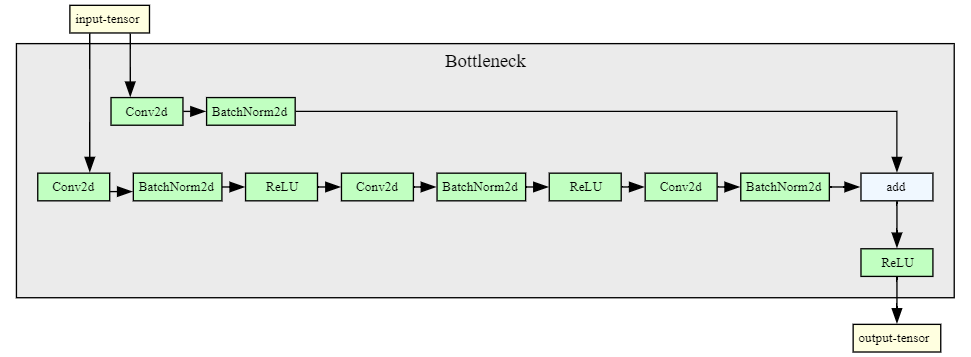
\includegraphics[width=15cm]{../images/resnet50_architecture_bottleneck.png}
    \caption{Architecture of Resnet50 bottleneck}
   \label{fig:resnet50_architecture_bottleneck}
    \end{center}
\end{figure}

\subsection{ViT-T/16}
Figure~\ref{fig:vit_t16_architecture}.

\begin{figure}[H]
    \begin{center}
    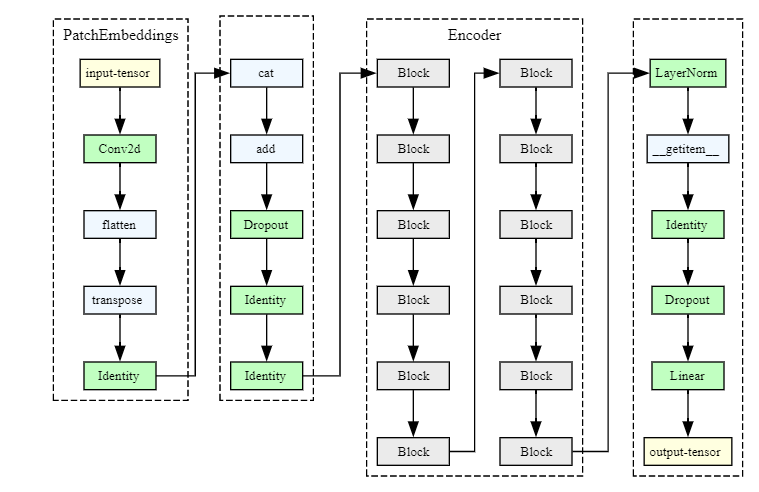
\includegraphics[width=15cm]{../images/vit_t16_architecture.png}
    \caption{Architecture of ViT-T/16}
   \label{fig:vit_t16_architecture}
    \end{center}
\end{figure}

Figure~\ref{fig:vit_t16_architecture_block}.

\begin{figure}[H]
    \begin{center}
    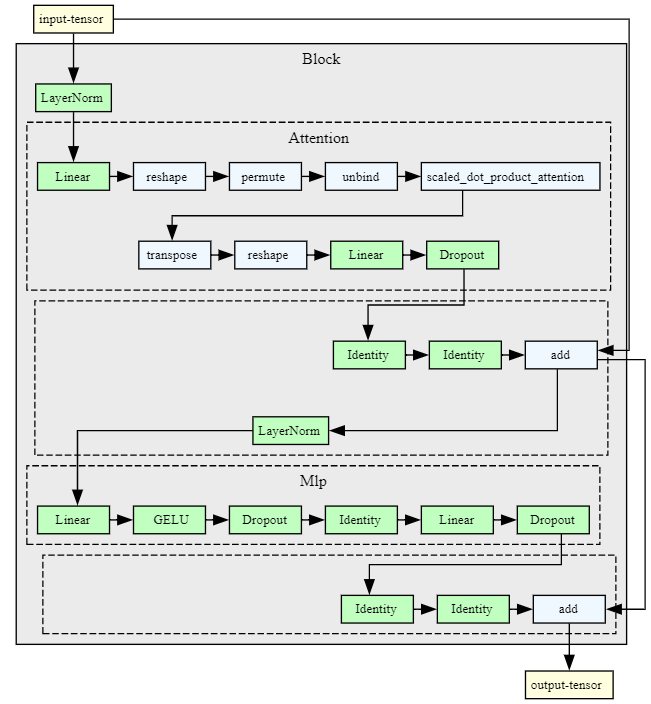
\includegraphics[width=15cm]{../images/vit_t16_architecture_block.png}
    \caption{Architecture of ViT-T/16 block}
   \label{fig:vit_t16_architecture_block}
    \end{center}
\end{figure}

% DINO
% Teacher / Student
